% Chapter 4: Artificial Intelligence Features
\chapter{Artificial Intelligence Features}

\chapterquote{Artificial intelligence is the new electricity.}{Andrew Ng}

\section*{Introduction}
\addcontentsline{toc}{section}{Introduction}

This chapter explores the integration of artificial intelligence capabilities within our real estate platform. We have developed four distinct AI models, each addressing specific needs within the ecosystem. These models collectively enhance user experience, improve decision-making processes, and provide valuable insights to various stakeholders in the real estate market.

The AI features presented in this chapter represent a significant competitive advantage for our platform, enabling more accurate property valuations, personalized recommendations, intelligent assistance, and efficient administrative operations. Each model has been carefully designed to solve real-world challenges faced by users interacting with real estate data and transactions.

\section{AI Development Overview}
\subsection{Technology Stack}


\subsection{Data Preprocessing Pipeline}
\subsubsection{Feature Engineering}


\subsubsection{Dataset Creation}


\subsection{Knowledge Base Construction}
\subsubsection{Information Extraction}


\subsubsection{Knowledge Organization}

\section{Data Collection and Scraping}
\subsection{Overview}
This section details the data collection processes implemented to gather the real estate market data required for our AI models. Effective data acquisition is a critical foundation for the AI capabilities implemented in our platform.

\subsection{Real Estate Data Scraping}
\subsubsection{Data Sources}
We implemented automated scraping systems to collect real estate data from various sources:
\begin{itemize}
    \item Real estate listing websites such as PropertyStar Tunisia \cite{PropertyStarTunisia} for comprehensive property listings and pricing data
    \item Property transaction records from public databases
    \item Real estate market reports and analytics platforms
    \item RE/MAX Tunisia \cite{RemaxTunisia} for detailed property valuation data in both sale and rental markets
    \item Al-Mindhar \cite{AlMindhar} for blog content related to legal aspects, investment strategies, and real estate regulations in Tunisia to train knowledge-based AI assistants
\end{itemize}
\newpage
\subsubsection{Scraping Architecture}
\begin{figure}[htbp]
    \centering
    % Placeholder for a diagram of the scraping workchart
    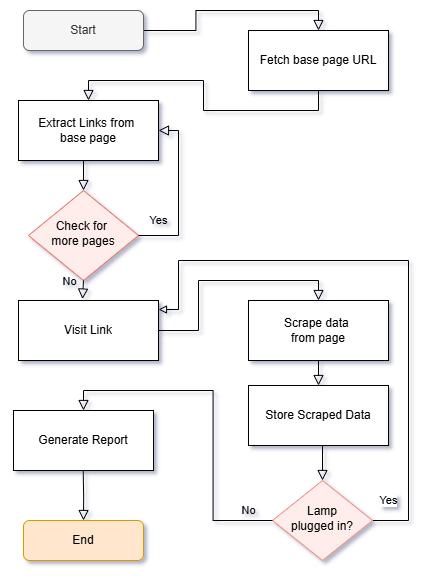
\includegraphics[width=0.55\textwidth]{images/workchartscraper.png}
    \caption{Data Scraping workchart}
    \label{fig:scraping-workchart}
\end{figure}

Our scraping system uses a distributed architecture with the following components:
\begin{itemize}
    \item Rate-limiting and request throttling to respect website policies
    \item Scheduled jobs for regular data updates
    \item Data validation and cleaning pipelines
\end{itemize}

\subsection{Data Storage and Management}
\subsubsection{Database Schema}
The collected data is stored in a structured database with the following key entities:
\begin{itemize}
    \item Property listings (with pricing history)
    \item Location data (neighborhoods, cities, regions)
    \item Property features and amenities
    \item Transaction records and market trends
\end{itemize}

\subsubsection{Data Versioning and Updates}
To maintain data quality and currency, we implemented:
\begin{itemize}
    \item Automated data refresh cycles for each source
    \item Version control for dataset updates
    \item Conflict resolution for data from multiple sources
    \item Data quality monitoring and alerting
\end{itemize}

\section{Property Valuation Prediction Model}
\subsection{Overview and Objectives}
The property valuation prediction model is designed to estimate both the market value and potential rental income for real estate properties. This provides investors with crucial information to make informed investment decisions.

\subsection{Model Architecture and Training Process}
\subsubsection{Model Selection}
After evaluating multiple approaches, we implemented:


\subsubsection{Training Methodology}


\subsection{Prediction Capabilities}


\subsection{Performance Metrics and Evaluation}


\subsection{Integration with Property Listings}
\subsection{Limitations and Future Improvements}

\section{Real Estate Assistant}
\subsection{Purpose and Capabilities}
\subsection{Conversational Interface Design}
\subsection{Legal Advisory Capabilities}
\subsection{Investment Insights Generation}
\subsection{Interaction Design and User Experience}
\subsection{Compliance and Information Accuracy}

\section{Role-Based Backoffice Agent}
\subsection{System Architecture}
\subsection{Database Integration and Access Control}
\subsection{Role-Based Permission Framework}
\subsection{Query Processing Pipeline}
\subsection{Response Generation and Formatting}
\subsection{Security and Privacy Considerations}

\section{Investor-Focused Recommendation System}
\subsection{Recommendation Algorithm Design}
\subsection{User Profiling and Preference Learning}
\subsection{Investment Criteria Matching}
\subsection{Integration with Mobile Platform}
\subsection{Performance Evaluation}
\subsection{Personalization and Adaptation Mechanisms}





